\section{Introduction}
\label{s_motive}

In the 70 years since nuclear bombs were dropped on Hiroshima and Nagasaki, the knowledge and technology required to make these weapons has proliferated around the globe. There are now nine states that have developed their own nuclear weapons, as well as many others who have the capability, if not the motivation, to do so\cite{feiveson_unmaking_2014}.  
%% I'm not thrilled with the implications of this sentence that all knowledge to build a bomb comes with
%% adoption of nuclear energy.  I'm not sure there is a better way without changing the paragraph to pivot
%% from bombs to energy in a different way.
Moreover, this knowledge will continue to spread as climate change change further tilts the scales such that the benefits of nuclear power outweigh the risks \cite{mooney_why_2014}.
%% The closing sentence of this paragraph is a characterization that I'm more comfortable with.
China is already investing heavily in nuclear power, planning to triple its generating capacity from 19GWe to 58GWe by 2020  \cite{_china_2014}.  As climate change becomes increasingly important with respect to national security, the perception of the risks inherent to nuclear energy is decreasing and states are embracing nuclear energy as a reliable large-scale source of carbon-neutral energy.  However, the expansion of nuclear power amplifies nuclear security concerns, because the same technologies used to produce nuclear fuel can also be exploited in the pursuit of nuclear weapons.


\subsection{Sensitive Parts of the Nuclear Fuel Cycle}

Two nuclear technologies are of of particular concern for proliferation, uranium enrichment and plutonium reprocessing.  Uranium enrichment is required for the once-through fuel cycles that are dominant around the world today, and used exclusively in the \gls{US}.  A once-through fuel cycle includes a source of natural uranium such as a mine, and is comprised of non-fissile 99.3\% $^{238}U$ and only 0.7\% fissile $^{235}U$. Concentrations of 3-5\% fissile $^{235}U$ are typical for fueling a nuclear power reactor.  
%% could add a sentence on research reactors and 20%, but it gets complicated since many still use HEU
Enrichment facilities are used to increase the concentration of $^{235}U$ from natural stock to the desired amount.  Fuel is then burned in a nuclear reactor and the remaining material, which includes the majority of the original $^{238}U$, as well as short- and long-lived fission products, and $\sim$1\% Pu (239 and 240), is then stored as waste.  The enrichment technique is a poliferations concern because it can be used to increase the concentration of $^{235}U$ up to the 90\% or more typically used to make a nuclear weapon\cite{_military_2014}.
%% There is much debate about making weapons out of lower enrichments, probably not worth including here.

Plutonium reprocessing is a proliferation concern because the technique can be used either to make recycled fuel or to make weapon-grade fissile material.  Several countries are developing nuclear reactors that can accomodate recycled fuel, providing the possibility of creating a closed fuel cycle\cite{_processing_2015}.  Recycled fuel is plutonium-based rather than uranium-based, and is made by separating the components of spent uranium fuel to extract the plutonium concentrations of fissile $^{239}Pu$ of approximately 50\%.  This material is generally  blended with uranium to make \gls{MOX} fuel.  Specially designed irradiation of uranium fuel can produce a plutonium component with $^{239}Pu$ concentrations up to 93\%, known as \gls{WGP}. However, fuel cycles with the capability to burn \gls{MOX} fuel are advangteous because \gls{WGP} from decommissioned nuclear weapons can be down-blended into \gls{MOX}, which reduces the amount of \gls{SNM} that must be safeguarded.  Reprocessessing has been considered at several times over the past half-century.  However, a host of political, economic, environmental and strategic concerns have pushed the issue of reprocessing out of the technical realm and it has become a contentious political topic\cite{rossin_policy_????}.  Currently the \gls{US} is pursuing only basic science research in this field \cite{editorial_adieu_2009}.
%% Do you want to mention currently-under-construction US MOX facility for converting WGP to commercial MOX fuel?
%% It may never be completed, though.

\subsection{Use of Treaties to Curtail Proliferation}

While it has not proven possible to prevent the spread of nuclear knowledge entirely, international treaties have been used in an attempt to minimize it.  The \gls{NPT}, which has been signed by 190 states including the original five nuclear weapons states, has codified a set of rules and norms for allowing the peaceful pursuit of nuclear energy\cite{_treaty_????}.  The \gls{NPT} created the \gls{IAEA}, whose role is to verify compliance with the treaty by periodically inspecting facilities related to nuclear technology.  Other relevant treaties include \gls{CTBT}, which placed a moratorium on testing nuclear weapons, and the \gls{START} in which the \gls{US} and Russia agreed to nuclear arms reductions.\TODO{citations}
%% CTBT has not yet entered into force.

These treaties have done much to prevent the spread of nuclear weapons knowledge, but they do not address the production capabilities of states that already posess nuclear weapons.
%% These treaties are not designed to prevent the spread of nuclear knowledge, just nuclear weapons knowledge.
A potential \gls{FMCT} would place limits on the amount of \gls{SNM} each weapons state could stockpile, possibly including current stockpiles in addition to future production.
%% FMCT would limit (cut-off) production of (waepons-grade) fissile material
%% for all countries, not just weapons states.
However, a major unresolved issue is the difficulty of developing verification techniques that can reliably confirm that nuclear material is not being produced \cite{_fissile_2013}.  Furthermore, making measurements of nuclear material for treaty verification is itself a sensitive issue, as even collecting the spectra of a material to confirm its authenticity can potentially expose sensitive information to the inspecting party\cite{glaser_zero-knowledge_2014}. Particularly if non-weapon states are to contribute to treaty verification, it is important to prevent the further dissemination of nuclear weapons knowledge.

\begin{figure}%[htbp!]
\begin{center}
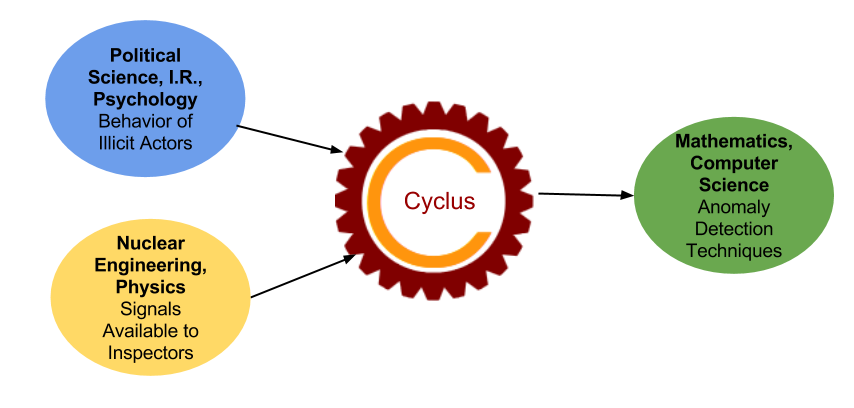
\includegraphics[natwidth=162bp,natheight=227bp, scale=0.5]{./figs/cyclus_interdiscipline.png}
\end{center}
\caption{The \Cyclus nuclear fuel cycle simulator provides a testbed to integrate innovations in treaty verification across many disciplines.}
\label{fig:cyclus_diagram}
\end{figure}

An effective treaty verification regime must synthesize knowledge from the realms of political science, international relations, nuclear physics and engineering, and even behavioral psychology.  A nuclear fuel cycle simulator such as \Cyclus, designed to track the detailed flow of nuclear material among different facilities, provides a framework in which to integrate these disparate fields.  Figure \ref{fig:cyclus_diagram} illustrates  the role of a fuel cycle simulator in combining models of the social-behavioral interactions between actors with the development of innovative detection modalities and signal processing techniques to provide insights into proposed verification approaches.  At a systems level, a fuel cycle simulator can be used to frame test scenarios as responses to stimuli. That is, even if not all of the specific details are available, simulations can incorporate response behaviors to illucidate the strengths and weaknesses of various verification strategies.


